\chapter{Cronograma de execução do projeto}

Como mostra a Fig. \ref{crono}, o plano de execução para o desenvolvimento do sPHENIX-MVTX tem a duração total de 3 anos (2020 - 2023), onde a produção dos dispositivos e a integração dos diversos componentes será executada. Neste contexto, como ilustra a seta em laranja na Fig. \ref{crono}, este projeto terá a duração inicial de um ano com início em 2021 e término em 2022, podendo claramente ser estendido de acordo com os compromissos assumidos durante esse período e a disponibilidade de recursos.
\\
\\
\begin{figure}[!h]
\centering
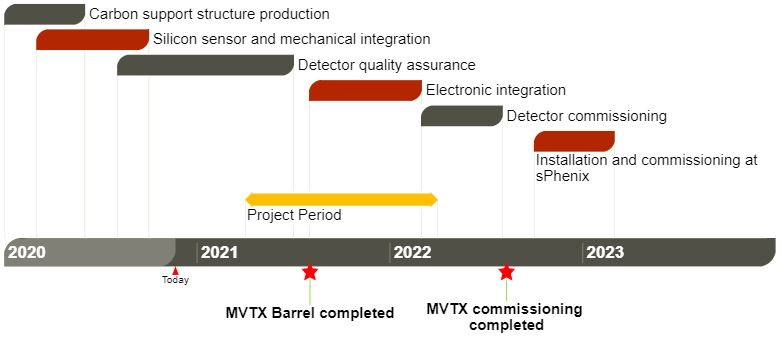
\includegraphics[width=15.0cm]{assets/cronograma.JPG}
\caption{Cronograma mostrando o planejamento para o desenvolvimento do MVTX. Os principais \textit{milestones} do projeto são mostrados em sua linha do tempo representados pelas estrelas em vermelho.}
\label{crono}
\end{figure}

Durante este período, o cronograma de desenvolvimento prevê o estabelecimento da infraestrutura para executar as medidas dos parâmetros de qualidade do sPHENIX-MVTX e sua integração com a eletrônica de aquisição de dados. Essas duas fases são importantes pois permitirá o desenvolvimento de atividades relacionadas com a caracterização do MVTX e seus diversos componentes, bem como a sua integração com o sistema de aquisição de dados, corroborando com os objetivos propostos neste documento. 

Por fim, os principais pontos do projeto de construção do sPHENIX-MVTX são mostrados em sua linha do tempo. De acordo com este cronograma, é importante destacar que o dispositivo estará completamente integrado em 2022.

